\documentclass{article}

\usepackage[heading=true]{ctex}
\usepackage[backref]{hyperref}
\usepackage{filecontents}
\usepackage{float}
\usepackage{graphicx}
\usepackage{geometry}
\usepackage{dirtree}
\usepackage{listings}
\usepackage{xcolor}
\usepackage{qtree}

\ctexset{
    section={
        number=\chinese{section},
        format+=\raggedright
    }
}
\geometry{a4paper, scale=0.8}

\definecolor{codegreen}{rgb}{0,0.6,0}
\definecolor{codegray}{rgb}{0.5,0.5,0.5}
\definecolor{codepurple}{rgb}{0.58,0,0.82}
\definecolor{backcolour}{rgb}{0.98,0.98,0.98}

\lstdefinestyle{lststyle}{
    backgroundcolor=\color{backcolour},
    commentstyle=\color{codegreen},
    keywordstyle=\color{magenta},
    numberstyle=\tiny\color{codegray},
    stringstyle=\color{codepurple},
    basicstyle=\ttfamily\small,
    breakatwhitespace=false,
    breaklines=true,
    captionpos=b,
    keepspaces=true,
    numbers=left,
    numbersep=5pt,
    showspaces=false,
    showstringspaces=false,
    showtabs=false,
    tabsize=2
}

\lstset{style=lststyle}


\title{实验二: 卷积神经网络实现}
\author{1190200703 管健男}
\date{}


\begin{document}

\maketitle


\section{实验环境}

\subsection{软硬件环境}

\begin{table}[h]
    \centering
    \begin{tabular}{|c|c|}
        \hline
        \textbf{OS}      & Linux 5.17.5-arch1-1 x86\_64 GNU/Linux \\
        \textbf{Python}  & 3.10.4                                 \\
        \textbf{Pytorch} & 1.11.0+cu113                           \\
        \hline
    \end{tabular}
    \caption{软件环境}
\end{table}

\begin{table}[h]
    \centering
    \begin{tabular}{|c|c|}
        \hline
        \textbf{CPU}        & 11th Gen Intel(R) Core(TM) i7-11700 @ 2.50GHz \\
        \textbf{GPU}        & NVIDIA GeForce RTX 3060 Lite Hash Rate        \\
        \textbf{GPU Driver} & 510.68.02                                     \\
        \textbf{CUDA}       & 11.6                                          \\
        \hline
    \end{tabular}
    \caption{硬件环境及驱动}
\end{table}

\subsection{源码目录结构}

源码目录结构如图\ref{src-dir}

\begin{figure}[H]
    \centering
    \begin{minipage}{0.5\linewidth}
        \dirtree{%
            .1 PatternRecognitionAndDeepLearningLabs.
            .2 DeepLearning.
            .3 lab2.
            .4 model.
            .5 AlexNet.ckpt.
            .4 dataloader.py.
            .4 main.py.
            .4 model.py.
            .4 trainer.py.
            .2 report.
            .3 LD-lab2.
            .4 LD-lab2.pdf.
            .4 LD-lab2.tex.
        }
    \end{minipage}
    \caption{源码目录结构}
    \label{src-dir}
\end{figure}

要进行训练并保存模型,只需修改main.py中load\_model为False,并在
PatternRecognitionAndDeepLearningLabs/DeepLearning/lab2目录下
运行python main.py。
要直接使用已有模型,只需修改main.py中load\_model为True即可。

\section{实验内容}

\subsection{读取数据}

由于Caltech101官方网站更新而pytorch的下载链接未更新,因此自动下载时会出现404报错。
手动下载数据即可,DataLoader模块可以自动校验。

\subsection{构建模型}

AlexNet模型结构如图\ref{alexnet}。

\begin{figure}[H]
    \centering
    \includegraphics[width=0.8\textwidth]{figures/alexnet.png}
    \caption{AlexNet模型结构}
    \label{alexnet}
\end{figure}

按照此结构,利用pytorch构造模型即可。注意原模型由于算力不足,将整个模型分为两路,
而在本次实验中,将这两路合并为了一路。

\begin{figure}[H]
    \centering
    \begin{minipage}{\textwidth}
        \centering
        \lstset{numbers=left,xleftmargin=2em,breaklines,language=Python, aboveskip=0pt,belowskip=0pt}
        \lstinputlisting[firstline=10,lastline=13,firstnumber=10]{model.py}
        \lstinputlisting[firstline=14,lastline=14,firstnumber=14,backgroundcolor=\color{orange!30}]{model.py}
        \lstinputlisting[firstline=15,lastline=18,firstnumber=15]{model.py}
        \lstinputlisting[firstline=19,lastline=19,firstnumber=19,backgroundcolor=\color{orange!30}]{model.py}
        \lstinputlisting[firstline=20,lastline=22,firstnumber=20]{model.py}
        \lstinputlisting[firstline=23,lastline=23,firstnumber=23,backgroundcolor=\color{orange!30}]{model.py}
        \lstinputlisting[firstline=24,lastline=27,firstnumber=24]{model.py}
        \lstinputlisting[firstline=28,lastline=28,firstnumber=28,backgroundcolor=\color{orange!30}]{model.py}
        \lstinputlisting[firstline=29,lastline=31,firstnumber=29]{model.py}
        \lstinputlisting[firstline=32,lastline=32,firstnumber=32,backgroundcolor=\color{orange!30}]{model.py}
        \lstinputlisting[firstline=33,lastline=36,firstnumber=33]{model.py}
        \lstinputlisting[firstline=37,lastline=37,firstnumber=37,backgroundcolor=\color{orange!30}]{model.py}
        \lstinputlisting[firstline=38,lastline=41,firstnumber=38]{model.py}
        \lstinputlisting[firstline=42,lastline=42,firstnumber=42,backgroundcolor=\color{orange!30}]{model.py}
        \lstinputlisting[firstline=43,lastline=46,firstnumber=43]{model.py}
        \lstinputlisting[firstline=47,lastline=47,firstnumber=47,backgroundcolor=\color{orange!30}]{model.py}
        \lstinputlisting[firstline=48,lastline=49,firstnumber=48]{model.py}
    \end{minipage}
    \caption{模型(前半部分)}
\end{figure}

\begin{figure}[H]
    \centering
    \begin{minipage}{0.8\textwidth}
        \centering
        \lstset{numbers=left,xleftmargin=2em,breaklines,language=Python, aboveskip=0pt,belowskip=0pt}
        \lstinputlisting[firstline=51,lastline=51,firstnumber=51]{model.py}
        \lstinputlisting[firstline=53,lastline=53,firstnumber=53,backgroundcolor=\color{orange!30}]{model.py}
        \lstinputlisting[firstline=54,lastline=57,firstnumber=54]{model.py}
        \lstinputlisting[firstline=58,lastline=58,firstnumber=58,backgroundcolor=\color{orange!30}]{model.py}
        \lstinputlisting[firstline=59,lastline=62,firstnumber=59]{model.py}
        \lstinputlisting[firstline=63,lastline=63,firstnumber=63,backgroundcolor=\color{orange!30}]{model.py}
    \end{minipage}
    \caption{模型(后半部分)}
\end{figure}

\subsection{数据集处理}

使用sklearn.model\_selection中的train\_test\_split函数对数据集进行划分,
如图\ref{split}。训练集、验证集和测试集比例为8:1:1

\begin{figure}[H]
    \centering
    \begin{minipage}{\textwidth}
        \centering
        \lstset{numbers=left,xleftmargin=2em,breaklines,language=Python, aboveskip=0pt,belowskip=0pt}
        \lstinputlisting[firstline=31,lastline=31,firstnumber=31]{dataloader.py}
        \lstinputlisting[firstline=32,lastline=33,firstnumber=32,backgroundcolor=\color{orange!30}]{dataloader.py}
    \end{minipage}
    \caption{划分训练集、验证集、测试集}
    \label{split}
\end{figure}

\subsection{图片预处理}

对图片进行缩放,缩放到$256 \times 256$,
然后进行中心裁剪,使最后的图片尺寸为$224 \times 224$。
如图\ref{resize}。

\begin{figure}[H]
    \centering
    \begin{minipage}{\textwidth}
        \centering
        \lstset{numbers=left,xleftmargin=2em,breaklines,language=Python, aboveskip=0pt,belowskip=0pt}
        \lstinputlisting[firstline=42,lastline=43,firstnumber=42]{dataloader.py}
        \lstinputlisting[firstline=44,lastline=45,firstnumber=44,backgroundcolor=\color{orange!30}]{dataloader.py}
        \lstinputlisting[firstline=46,lastline=48,firstnumber=46]{dataloader.py}
    \end{minipage}
    \caption{划分训练集、验证集、测试集}
    \label{resize}
\end{figure}

\section{实验结果与分析}

调整训练次数epoch=30,数据批量batch\_size=20,使用tensorboard查看
训练集、开发集的acc和loss情况,如图
\ref{devacc}、\ref{devloss}、\ref{trainacc}、\ref{trainloss}所示。

\begin{figure}[H]
    \centering
    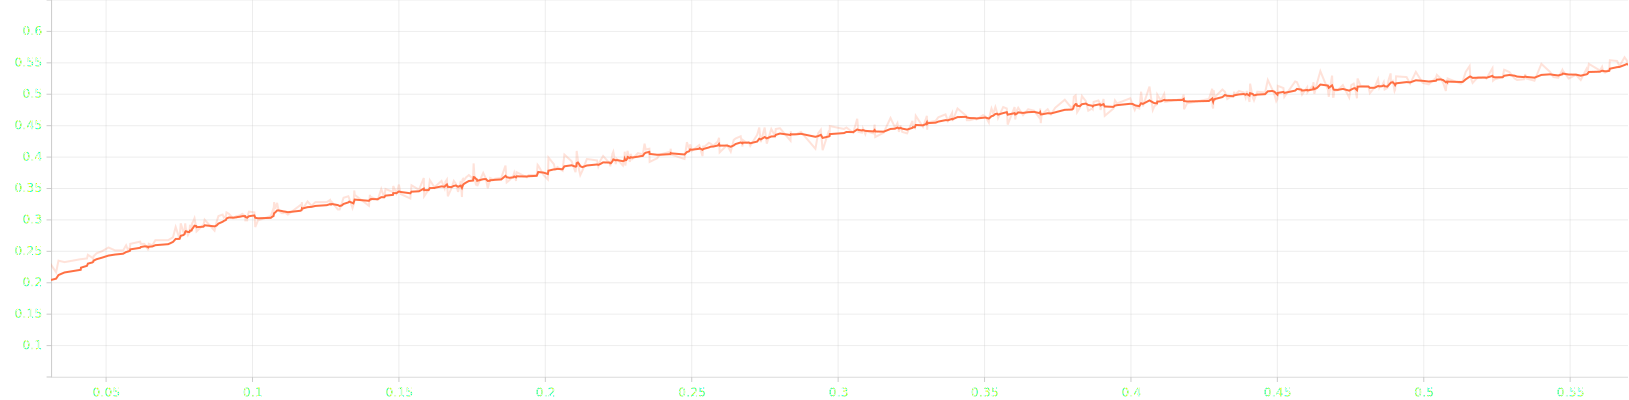
\includegraphics[width=0.8\textwidth]{figures/dev_acc.png}
    \caption{dev acc}
    \label{devacc}
\end{figure}

\begin{figure}[H]
    \centering
    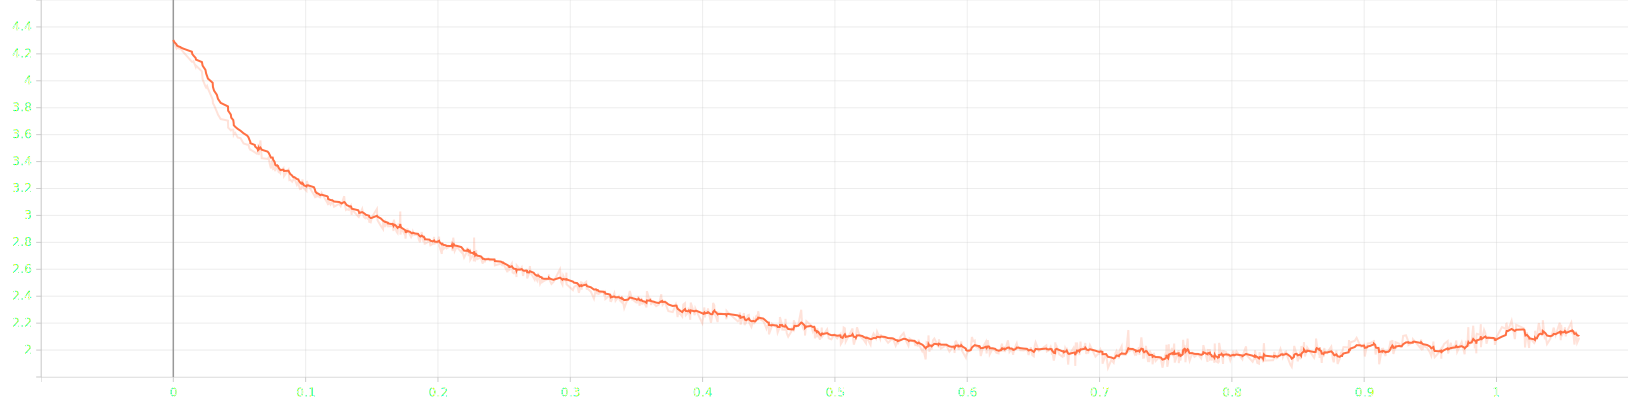
\includegraphics[width=0.8\textwidth]{figures/dev_loss.png}
    \caption{dev loss}
    \label{devloss}
\end{figure}

\begin{figure}[H]
    \centering
    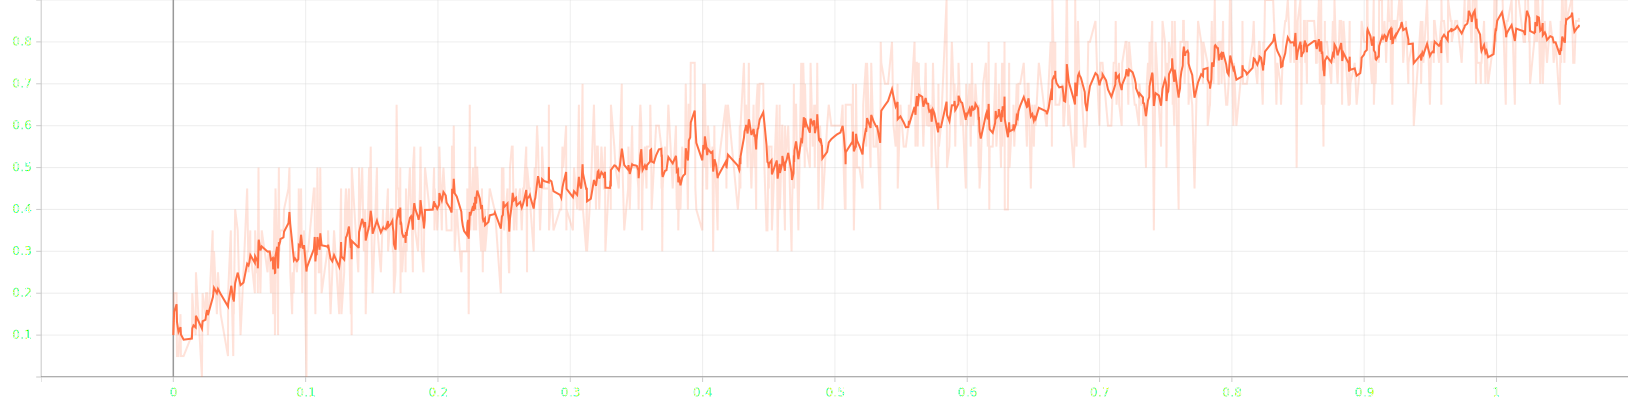
\includegraphics[width=0.8\textwidth]{figures/train_acc.png}
    \caption{train acc}
    \label{trainacc}
\end{figure}

\begin{figure}[H]
    \centering
    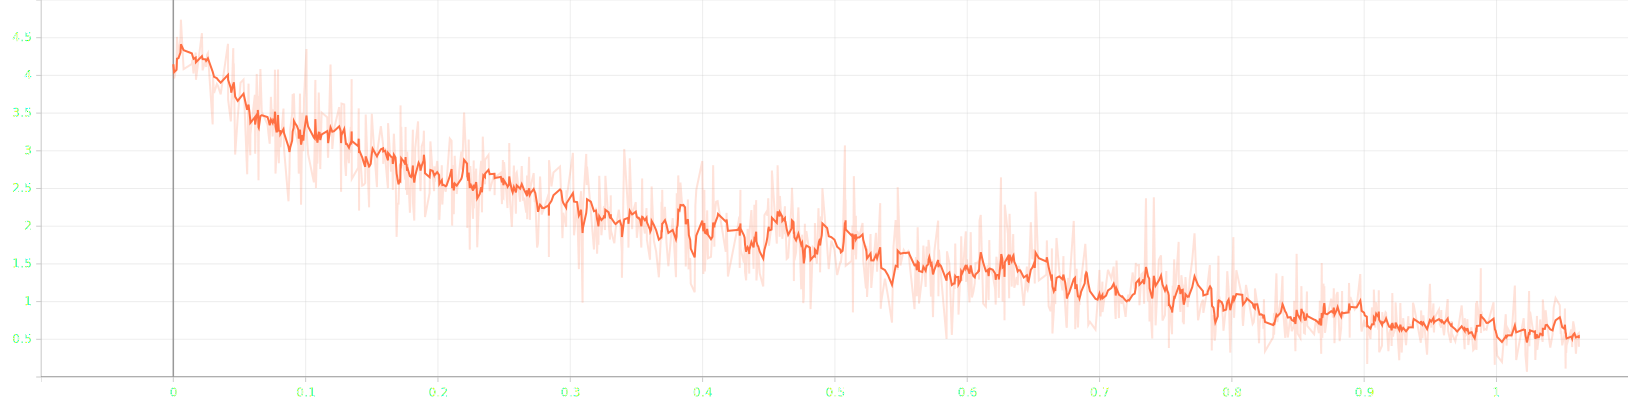
\includegraphics[width=0.8\textwidth]{figures/train_loss.png}
    \caption{train loss}
    \label{trainloss}
\end{figure}

在训练集、开发集、测试集上的各个acc和loss如表\ref{test}

\begin{figure}[H]
    \centering
    \begin{tabular}{lll}
        \hline
        \textbf{Data}        & \textbf{Acc} & \textbf{Loss} \\
        \hline
        Train        85.34\% & 0.51\%                       \\
        Dev          56.12\% & 2.13\%                       \\
        Test         58.51\% & 2.29\%                       \\
        \hline
    \end{tabular}
    \caption{各个数据集上的acc和loss}
    \label{test}
\end{figure}

\end{document}
